\documentclass[
	12pt,		%fonte padrão 12pt
	oneside,
	a4paper,
	chapter=TITLE,
	english,
	brazil,
	hidelinks
]{abntex2}

\usepackage{lmodern}
\usepackage[T1]{fontenc}
\usepackage[utf8]{inputenc}
\usepackage{indentfirst}
\usepackage{color}
\usepackage{graphicx}
\usepackage{microtype}
\usepackage[labelfont={bf},font=small,skip=0.5cm]{caption}

\usepackage{blindtext}

%\renewcommand{\familydefault}{\sfdefault}

\usepackage[alf]{abntex2cite}

\setlength{\parindent}{1.3cm}
\setlength{\parskip}{\onelineskip}
\setlength\afterchapskip{0cm}

\renewcommand{\ABNTEXchapterfont}{\fontseries{b}\selectfont} 
\renewcommand{\ABNTEXchapterfontsize}{\normalsize}

\renewcommand{\ABNTEXsectionfont}{\fontseries{b}\selectfont} 
\renewcommand{\ABNTEXsectionfontsize}{\normalsize}

\renewcommand{\cftchapterfont}{\ABNTEXchapterfont} 
\renewcommand{\cftsectionfont}{\fontseries{m}\selectfont} 

\renewcommand{\tocheadstart}{\ABNTEXchapterfont} 

\renewcommand{\tocprintchapter}{%
    \addtocontents{toc}{\cftsetindents{chapter}{0em}{2em}}}
\cftsetindents{section}{0em}{2em}
\setlength{\cftbeforechapterskip}{0em}

\addtocontents{toc}{\vspace{\onelineskip}}
%\cftsetindents{chapter}{0em}{2em}
%\cftsetindents{section}{0em}{2em}

\addtocontents{lof}{\vspace{\onelineskip}}
%\setlength{\abovecaptionskip}{0.1cm}
%\setlength{\belowcaptionskip}{0.1cm}

\addtocontents{lot}{\vspace{\onelineskip}}

\nobibintoc

\titulo{Produção de biogás em pequena escala a partir de lixo orgânico e rejeito animal}
\autor{
Adilson Barcelos Araujo RA 1830132\\
Henrique da Costa Bertolasio dos Santos RA 1834296 \\
Marcelo Rodrigues da Silva RA 1823767\\
Marcio de Souza Maia Junior RA 1819900\\
Osvalton Cílio Souza da Silva RA 1834284\\
Sandra dos Anjos Lopes RA 1833347\\
}
\local{Cubatão - SP}
\data{2019}
\orientador{Tutor: Carlos Eduardo de Freitas Garcia}
\instituicao{UNIVERSIDADE VIRTUAL DO ESTADO DE SÃO PAULO}
\preambulo{Relatório parcial para a disciplina de Projeto Integrador do curso de Engenharia da Computação da Universidade Virtual do Estado de São Paulo.}

\renewcommand{\imprimircapa}{%
\begin{capa}%
	\center
	\ABNTEXchapterfont\large \imprimirinstituicao
	\vfill
	\fontseries{m}\normalsize \imprimirautor
	\vfill
	\ABNTEXchapterfont\large \imprimirtitulo
	\vfill
	\fontseries{m}\normalsize\imprimirlocal\\
	\fontseries{m}\normalsize\imprimirdata
\end{capa}
}

\makeatletter 
\renewcommand{\folhaderostocontent}{
\begin{center}
	\ABNTEXchapterfont\large UNIVERSIDADE VIRTUAL DO ESTADO DE SÃO PAULO
	\vfill
	\ABNTEXchapterfont\large \imprimirtitulo
	\vfill
	\hspace{.45\textwidth} 
	\begin{minipage}{.5\textwidth} 
	\SingleSpacing 
	\fontseries{m}\normalsize\imprimirpreambulo
	\\[1\baselineskip]
	\fontseries{b}\normalsize\imprimirorientador
	\end{minipage} 
	\vfill
	\fontseries{m}\large\imprimirlocal\\
	\fontseries{m}\large\imprimirdata
\end{center}
}

\makeatletter
\setlength{\@fptop}{5pt} % Set distance from top of page to first float
\makeatother


\makeindex

\begin{document}

\selectlanguage{brazil}

\frenchspacing

\imprimircapa

\imprimirfolhaderosto*

%\setlength{\absparsep}{18pt} % ajusta o espaçamento dos parágrafos do resumo
\begin{resumo}\vspace*{-1.1cm}
\SingleSpacing Ao longo da história da humanidade muitas ações ambientalistas têm sido definidas por sequências práticas e percepções que atingem, até os dias atuais, ritmos diferentes ao mesmo tempo em que oferecem uma revolução capaz de conduzir toda a humanidade na mesma direção. Como prova da continuidade em buscar por ações que minimizem os impactos causados ao meio ambiente é fácil apontar o uso de várias fontes de energia renováveis, como é o caso do biogás. Um composto de metano (CH4) e dióxido de carbono (CO2), o biogás, um biocombustível produzido por meio de dejetos humanos, esterco, resíduos agrícolas, etc., têm tornado um grande incentivador para a geração de energia limpa em todo o mundo. E, na busca por opções ambientalmente corretas a destinação de resíduos a necessidade de ampliação e diversificação da matriz energética brasileira esse relatório busca por verificar a viabilidade da construção de biodigestores em pequena escala para a geração de biogás através da decomposição de lixo orgânico e rejeito animal. Valendo de uma revisão bibliográfica e estudo a campo, ao final, essa pesquisa espera esclarecer quais as técnicas e as tecnologias envolvidas na produção do biogás capazes de oferecer uma opção para a geração de energia limpa que seja ambientalmente correta e economicamente viável.

\textbf{Palavras-chave}: Biogás. Lixo orgânico. Rejeito animal. Adubo.
\end{resumo}

% resumo em inglês
%\setlength{\absparsep}{18pt} % ajusta o espaçamento dos parágrafos do resumo
\begin{resumo}[Abstract]\vspace*{-1.1cm}
\begin{otherlanguage*}{english}\SingleSpacing
Throughout the history of humanity many environmental actions have been defined by practical sequences and perceptions that reach, until the present day, diferente rhythms at the same time that they offer a revolution capable of leading all the humanity in the same direction. As proof of the continuity in searching for actions that minimize the impacts caused to the environment, it is easy to point out the use of several renewable energy sources, such as biogas. A compound of methane (CH4) and carbon dioxide (CO2), biogas, a biofuel produced through human waste, manure, agricultural waste, etc., have become a major incentive for clean energy generation worldwide. And, in the search for environmentally correct options for waste disposal, the need to expand and diversify the Brazilian energy matrix, this report seeks to verify the feasibility of the construction of small scale biodigesters for the generation of biogas through the decomposition of organic waste and animal waste. In the end, this research hopes to clarify which techniques and technologies are involved in biogás production. capable of offering an option for the generation of clean energy that is environmentally correct and economically viable.

\textbf{Keywords}: Biogas. Organic waste. Animal waste. Fertilizer.
\end{otherlanguage*}
\end{resumo}

\pdfbookmark[0]{\listfigurename}{lof}
\listoffigures*
\cleardoublepage

\pdfbookmark[0]{\listtablename}{lot}
\listoftables*
\cleardoublepage

\pdfbookmark[0]{\contentsname}{toc}
\tableofcontents*
\cleardoublepage

\textual

\pagestyle{simple}

\chapter{Introdução}

O interesse em fontes alternativas de energia é relativamente recente e vem crescendo rapidamente. Entre outras razões para esse interesse podemos citar o sistemático aumento no preço dos combustíveis fósseis e da energia elétrica. O impacto ambiental envolvido na produção e consumo destas fontes de energia, na forma dos gases de efeito estufa, também não pode ser ignorado. Uma dessas alternativas é o uso de lixo orgânico e rejeito animal para a produção de biogás.

O processo de produção de biogás a partir de resíduos orgânicos e dejeto animal já é conhecido há muito tempo (FERRAZ, 1980). O biogás gerado desta forma é composto por aproximadamente 60\% de gás metano (CH4) e 38\% de dióxido de carbono (CO2). A mistura gasosa obtida, por ser rica em metano, pode ser utilizada como combustível. Além disso, os resíduos da produção de biogás podem ser utilizados como adubo. O equipamento utilizado para a produção de biogás é chamado de biodigestor.

O presente relatório tem como objetivo checar a viabilidade técnica e econômica da construção e utilização de biodigestores em pequena escala, utilizando-se biodigestores de batelada compactos e construídos a partir de materiais simples e baratos. 

\section{Problemas e objetivos}

A investigação da viabilidade da construção e utilização de biodigestores em pequena escala pretende melhorar o entendimento da tecnologia envolvida na produção do biogás e tem como principais objetivos:

\begin{itemize}
\item Investigar os custos envolvidos na construção de um biodigestor;
\item Identificar a matéria prima utilizada na produção de biogás;
\item Quantificar a produção de biogás por unidade de matéria prima;
\item Verificar os possíveis problemas advindos da utilização de um biodigestor.
\end{itemize}

De acordo com Ferraz (1980, p. 20), biodigestores com 2 metros cúbicos são capazes de gerar 1100 litros de biogás por dia. A proposta deste presente relatório é verificar se há possibilidade de se construir um biodigestor ainda menor. Com menos de 1 metro cúbico de volume.

\section{Justificativa}

Com o aumento no custo da energia, é cada vez mais importante pesquisar novas fontes energéticas, de preferência fontes limpas e renováveis. A geração de biogás é barata pois usa como matéria prima o lixo orgânico e resíduos animais. Além disso, até mesmo os resíduos da produção do biogás podem ser reaproveitados.

Contudo, é necessário investigar mais a fundo a viabilidade técnica e econômica da produção de biogás em pequena escala por meio do uso de um biodigestor. 

Finalmente, é importante lembrar que o Brasil recebeu, ainda na década de 70, com a crise do petróleo, a tecnologia da digestão anaeróbica (PECORA, 2006). Portanto, a tecnologia já é bem conhecida, o que ajuda a diminuir os riscos.

\section{Consumo energético no estado de São Paulo}

No gráfico abaixo podemos verificar o consumo anual de energia elétrica e de petróleo no estado de São Paulo desde o ano de 2006 até 2017. A partir destes dados foi criada uma previsão baseada em uma tendência linear até o ano de 2025. De acordo com estas informações, o consumo anual de energia elétrica pode passar dos atuais 129.810.078 MWh para 151.885.615 MWh, um aumento significativo de 17\%. Já no caso do petróleo, o consumo pode aumentar 26\%, passando dos atuais 29.337 milhões de litros para 37.126 milhões de litros (SECRETARIA DE INFRAESTRUTURA E MEIO AMBIENTE DO ESTADO DE SÃO PAULO, 2018).

\vspace{0.8cm}

\begin{figure}[htb]
	\begin{center}
	    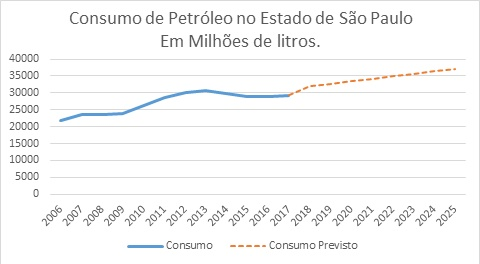
\includegraphics[scale=1.0]{consumo_petroleo_sp.jpg}
	\end{center}
	\vspace*{-0.5cm}
	\caption{\label{fig_graficooo}Consumo de petróleo no estado de São Paulo}
	%\legend{Fonte: \citeonline[p. 24]{araujo2012}}
\end{figure}

\begin{figure}[htb]
	\begin{center}
	    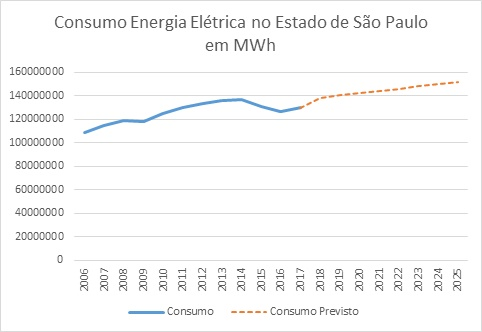
\includegraphics[scale=1.0]{consumo_eletricidade_sp.jpg}
	\end{center}
	\vspace*{-0.5cm}
	\caption{\label{fig_graficoooo}Consumo de de eletricidade no estado de São Paulo}
	%\legend{Fonte: \citeonline[p. 24]{araujo2012}}
\end{figure}



\chapter{Fundamentação teórica}

\section{Biodigestores}

Os equipamentos utilizados para a produção de biogás são chamados biodigestores. Eles são tanques fechados onde se obtém o gás metano a partir da fermentação de resíduos orgânicos na ausência de oxigênio.

Existem vários tipos de biodigestores, os mais usados são os contínuos e os de batelada (FERRAZ, 1980). No modelo contínuo, é introduzido o material orgânico misturado com água de maneira que o gás metano gerado é armazenado em um gasômetro. Dessa maneira o fluxo de gás é contínuo a medida em que o material orgânico é depositado. Os resíduos são então captados na saída e podem ser utilizados imediatamente. O modelo Indiano e o modelo Chinês são duas implementações diferentes, mas bastante utilizadas do biodigestor do tipo contínuo.

Já no sistema de biodigestor de batelada, o material orgânico é depositado uma só vez e só é removido após todo o gás ter sido utilizado. Este modelo é consideravelmente mais simples que o modelo contínuo.  

Os biodigestores contínuos e de batelada, são conhecidos coletivamente como biodigestores rurais.

\begin{citacao}
“Existem, atualmente uma gama muito grande de modelos de biodigestores, sendo cada um adaptado a uma realidade e uma necessidade de biogás, neste trabalho trataremos exclusivamente de biodigestores utilizados em pequenas propriedades no meio rural”.\cite{abntex2-wiki-como-customizar}
\end{citacao}

Estes são os biodigestores mais comuns e baratos em operação atualmente. O protótipo será construído com base no modelo de batelada.

\section{Biogás}

O biogás é uma mistura gasosa composta por aproximadamente 60\% de gás metano (CH4) e 38\% de dióxido de carbono (CO2). O metano é um gás combustível e pode ser utilizado como fonte energética.

O poder calorífico do biogás é da ordem de 5000 kcal/m3 quando misturado com o dióxido de carbono. Para colocar em perspectiva podemos compará-lo com o poder calorífico de outros combustíveis.

\begin{table}[htb]
\centering
\footnotesize
\begin{tabular}{ll}
\toprule
\multicolumn{2}{c}{\textbf{1$m^3$ de biogás equivale a:}} \\
\midrule \midrule
0,613L & Gasolina \\
\midrule 
0,579L & Querosene \\
\midrule 
0,553L & Óleo Diesel \\
\midrule 
0,454Kg & GLP (Gás liquefeito de petróleo) \\
\midrule 
1,428KW/h & Energia elétrica \\
\bottomrule
\end{tabular}%
\caption{Equivalência de poder calorífico}
\end{table}

1m3 de biogás equivale a:
0,613L	Gasolina
0,579L	Querosene
0,553L	Óleo Diesel
0,454Kg	GLP (Gás liquefeito de petróleo)
1,428KW/h	Energia elétrica
Tabela 1 – Equivalência de Poder Calorífico
O biogás gerado pode ser utilizado diretamente para alimentar fogões ou motores a combustão (como os utilizados em geradores).

\section{Biomassa}

A biomassa é a matéria prima utilizada na produção do biogás. Podem ser divididos em:

\begin{itemize}
\item Esterco (de gado, de suínos, de aves, etc.);
\item Resíduo orgânico residencial;
\item Efluentes (esgoto).
\end{itemize}

É necessário que na fase inicial de operação do biodigestor, seja utilizada uma quantidade de fezes para garantir a presença de bactérias metagênicas, sem as quais o biogás não pode ser produzido (FERRAZ, 1980).

\section{Fatores que afetam o consumo e a produção de gás}

O transporte do biogás não pode ser feito para longas distâncias sem o auxílio de um compressor pois o gás é armazenado em baixa pressão.

A produção do biogás é otimizada em temperaturas ao redor dos 35ºC. Temperaturas abaixo dos 15ºC inibem drasticamente o processo.

\section{Biofertilizante}

Como foi dito, os resíduos da produção de biogás podem ser utilizados como fertilizantes. O nitrogênio é quase que totalmente conservado no processo e o material pode ser utilizado imediatamente.

\section{Aplicação das disciplinas estudadas no projeto integrador}

A disciplina de Produção de Textos foi fundamental para a elaboração deste relatório, fornecendo técnicas importantes de leitura e escrita. Outra disciplina importante foi a de Metodologia Científica, por meio da qual conseguimos entender o processo de construção dos trabalhos científicos. Inglês foi decisivo na hora de consultar referências na língua inglesa. Já a disciplina de Física nos permitiu compreender o comportamento dos gases gerados pelo processo de geração de biogás. Outra matéria fundamental foi a de Introdução à Informática que nos mostrou os principais aplicativos utilizados no meio científico para a confecção de trabalhos acadêmicos. Finalmente cálculo foi responsável por sermos capazes de apreciar as passagens mais complicadas do processo.

\chapter{Materiais e métodos empregados}

Foi utilizado o processo de pesquisa bibliográfica na plataforma SCIELO e Google Scholar. Biogás e biodigestor foram as palavras chaves escolhidas para a pesquisa.

\chapter{Análise e discussão dos resultados}

A partir do estudo do processo de produção de biogás através da digestão anaeróbica o grupo discutiu possíveis implementações e custos envolvidos. Foi criado então um cronograma para o detalhamento da proposta e a possível construção de um protótipo para uma análise mais profunda. 

O protótipo a ser construído e estudado será baseado no modelo criado por três estudantes de Engenharia Civil e Engenharia de Produção da Universidade Federal de Alagoas devido ao seu baixo custo e facilidade de construção (NOSSACIENCIA, 2018).
\vspace{0.2cm}

\begin{figure}[htb]
	\begin{center}
	    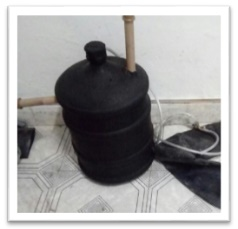
\includegraphics[scale=1.0]{prototipo.jpg}
	\end{center}
	\vspace*{-0.5cm}
	\caption{\label{fig_grafico}Protótipo}
	%\legend{Fonte: \citeonline[p. 24]{araujo2012}}
\end{figure}

\chapter{Introdução}

\blindtext

\section{Justificativa}

\Blindtext

\chapter{Desenvolvimento}

\blindtext

\begin{citacao}

\blindtext\cite[5.3]{NBR10520:2002}.

\end{citacao}

\begin{figure}[htb]
	\begin{center}
	    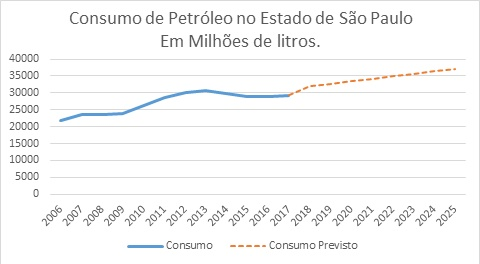
\includegraphics[scale=1.0]{consumo_petroleo_sp.jpg}
	\end{center}
	\caption{\label{fig_grafico1}Consumo de petróleo no estado de São Paulo}
	%\legend{Fonte: \citeonline[p. 24]{araujo2012}}
\end{figure}


\section{Justificativa}

\Blindtext

\begin{figure}[htb]
	\caption{\label{fig_graficoy}Consumo de de eletricidade no estado de São Paulo}
	\begin{center}
	    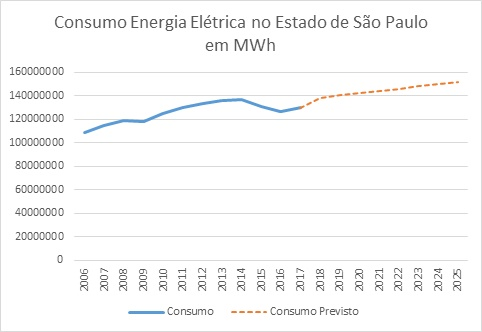
\includegraphics[scale=1.0]{consumo_eletricidade_sp.jpg}
	\end{center}
	%\legend{Fonte: \citeonline[p. 24]{araujo2012}}
\end{figure}

\chapter{Conclusão}

\blindtext

\begin{figure}[htb]
	\caption{\label{fig_graficox}prototipo}
	\begin{center}
	    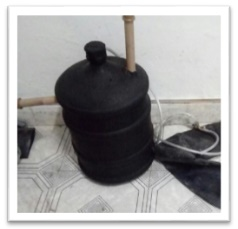
\includegraphics[scale=1.0]{prototipo.jpg}
	\end{center}
	%\legend{Fonte: \citeonline[p. 24]{araujo2012}}
\end{figure}

\section{Custos}

\Blindtext

\postextual

\bibliography{bib}

\end{document}
